\chapter{Metodo proposto}
\label{cha:metodo_proposto}

Nel terzo capitolo viene presentata la metodologia seguita per l'analisi di immagini condivise tramite la piattaforma WhatsApp con l'obiettivo di risalire al dispositivo e al sistema software impiegato (Fig.~\ref{fig:metodo}). Come prima cosa sarà descritto il modo in cui è stato creato SHADE, dataset appositamente realizzato per questo scopo (\ref{sec:SHADE}). In seguito esamineremo due metriche, \textit{Mean Square Error} (MSE) e \textit{Peak Signal-to-Noise Ratio} (PSNR), utilizzate per un'analisi di tipo qualitativo delle immagini (\ref{sec:mse_psnr}). Si passerà poi a descrivere la fase di estrazione di \textit{feature} (\ref{sec:estr_feat}) e la loro visualizzazione grazie alla creazione di mappe Isomap (\ref{sub:isomap}). Come ultimo passaggio, illustreremo i due metodi utilizzati per la classificazione (\ref{sec:classificazione}). Tutte le fasi qui riportate sono state accompagnate dalla scrittura di codice Python per l'analisi, la visualizzazione e la classificazione delle immagini.

\begin{figure}[h!]
    \centering
    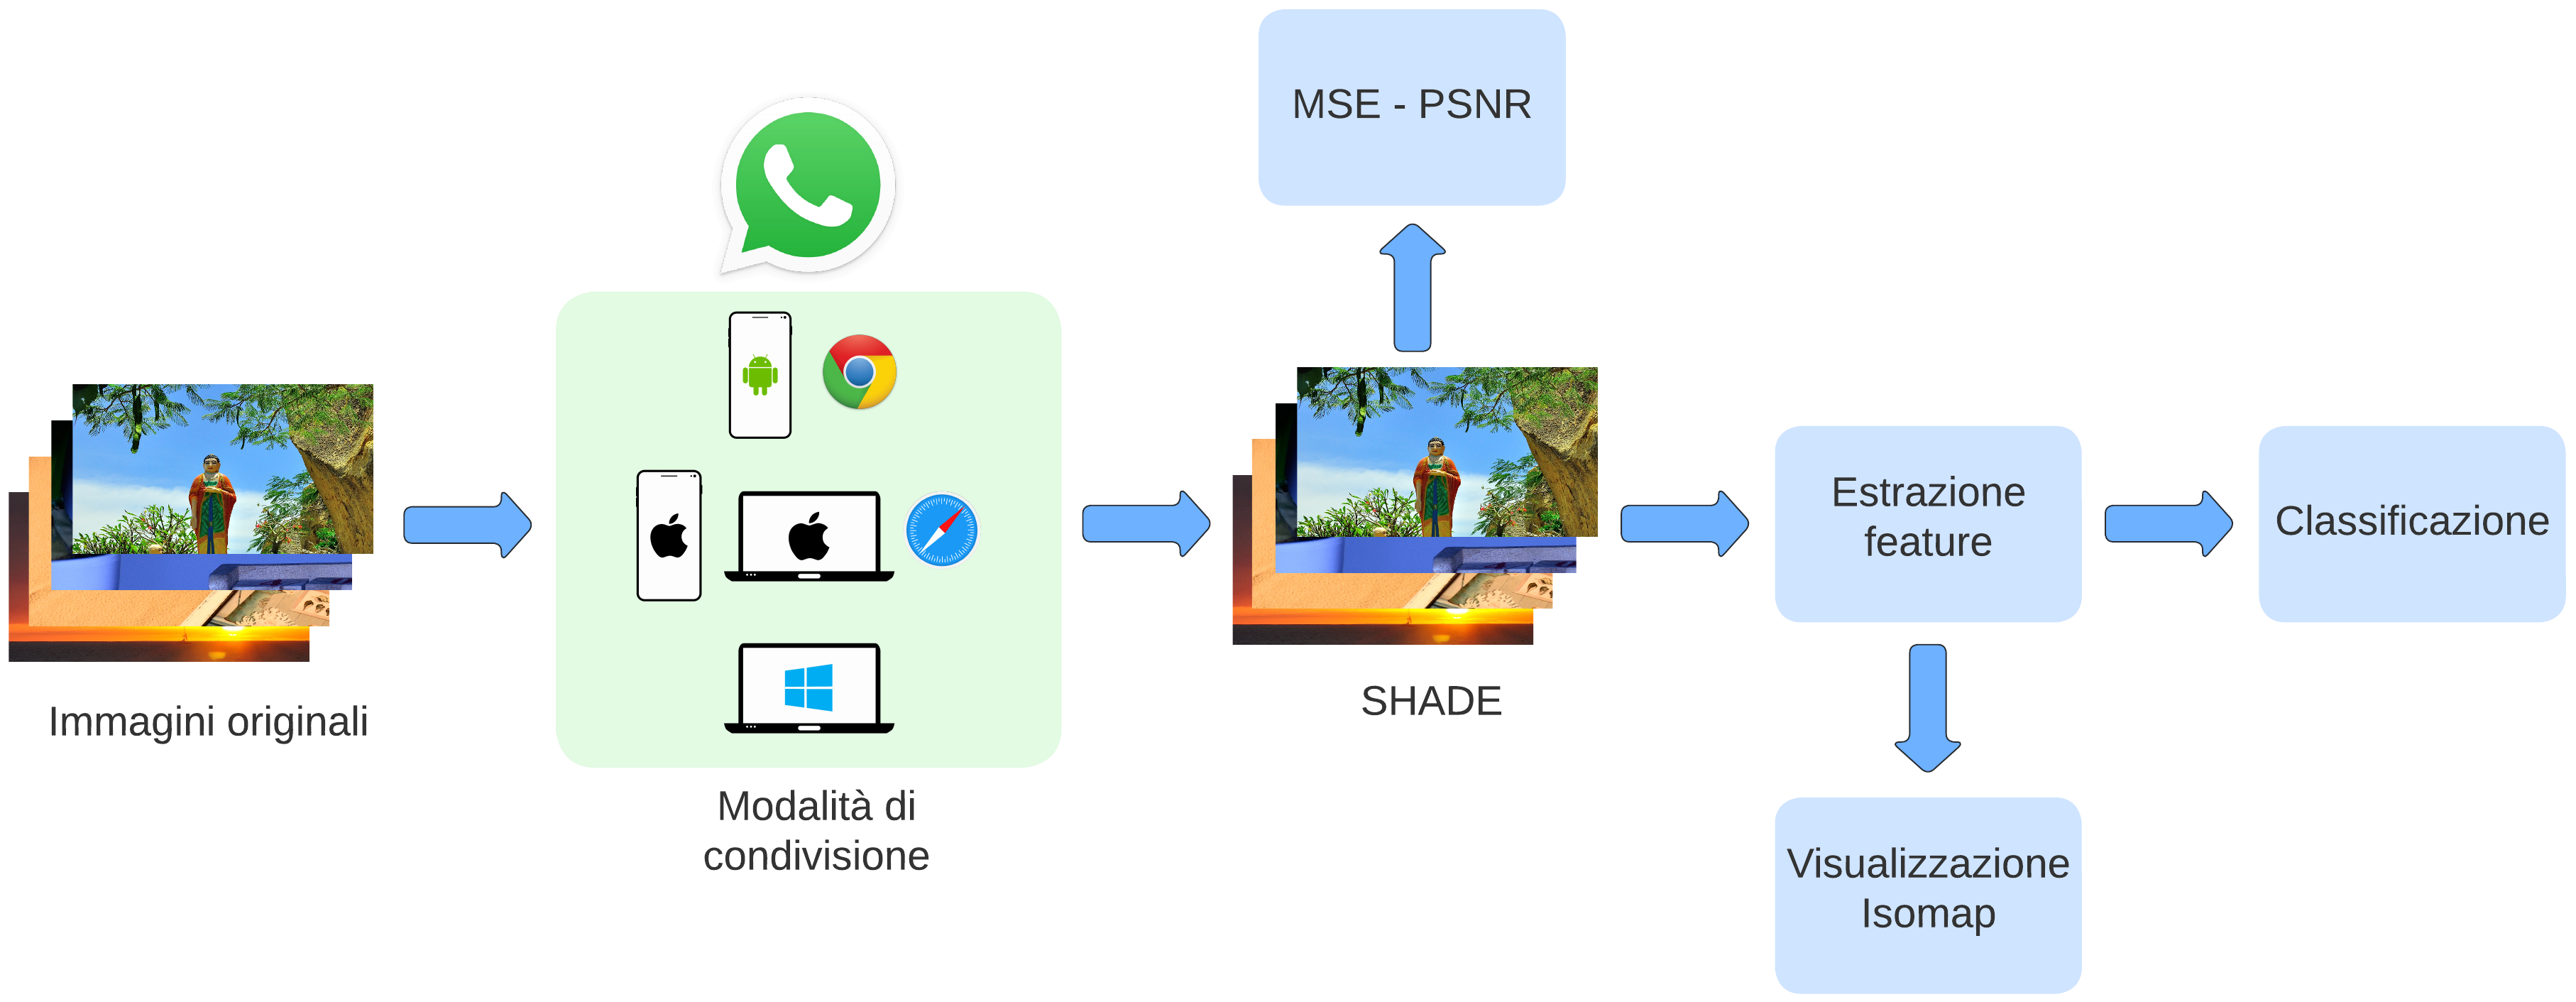
\includegraphics[width=\columnwidth]{Immagini/metodo_proposto.png}
    \caption{\textit{Pipeline} seguita per le analisi su SHADE}
    \label{fig:metodo}
\end{figure}

\section{SHADE}
\label{sec:SHADE}

Il processo di creazione di SHADE (acronimo di \textit{SHAring DEvice}) è partito da 50 immagini in formato RAW prese dal dataset RAISE. In maniera simile a quanto avvenuto per R-SMUD le immagini sono state ritagliate dall'angolo sinistro superiore per ottenere tre copie con le seguenti risoluzioni: $337\times600$, $1012\times1800$ e $1687\times3000$ con un \textit{aspect ratio} di $9:16$. Tutte le immagini ritagliate hanno poi subito una compressione JPEG utilizzando sei \textit{quality factor} differenti (QF = 50, 60, 70, 80, 90, 100) per un totale di 900 elementi ($50\times3\times6$).
La piattaforma social che abbiamo selezionato per la condivisione è WhatsApp ed è stata scelta per una serie di motivazioni: rappresenta uno dei più famosi social network per lo scambio di informazioni e mette a disposizione molteplici interfacce software (desktop, browser, mobile) per diversi sistemi operativi (Windows, Android, iOS) permettendo di studiarne i numerosi aspetti del suo funzionamento. Le modalità di condivisione prese in esame sono:\newpage

\begin{table}[h!]
    \normalsize
    \centering
    \begin{tabular}{ll}
        \textbf{Tag} & \textbf{Descrizione}\\
        \midrule
        \textit{ANDROID} & Applicazione mobile per Android\\
        \textit{APP-MAC} & Applicazione desktop per MacOS\\
        \textit{APP-WIN} & Applicazione desktop per Windows 10\\
        \textit{IPHONE} & Applicazione mobile per iOS\\
        \textit{WEB-IPAD} & Browser (Safari) per iPadOS\\
        \textit{WEB-MAC} & Browser (Safari) per MacOS\\
        \textit{WEB-WIN} & Browser (Chrome) per Windows 10\\
    \end{tabular}
\end{table}

Ognuna delle 150 immagini di partenza è stata condivisa sette volte attraverso i metodi sopra elencati e, per ogni \textit{quality factor}, altre sei volte. In questo modo il dataset finale è costituito da $150\times6\times7 = 6300$ elementi a cui si aggiungono le 900 immagini originali non condivise. 
Come nella fase di upload anche il download dei contenuti da WhatsApp è stato eseguito manualmente a causa della mancanza di API (\textit{Application Programming Interface}) gratuite che avrebbero permesso di gestire con maggiore facilità le immagini.  Durante il salvataggio queste vengono rinominate da WhatsApp con un pattern distintivo. Nel nome del file è possibile identificare quattro elementi riportati di seguito con un esempio:

\begin{equation}
    \underbrace{\vphantom{.jpeg} WhatsApp \ \ Image}_{nome} \ \ \underbrace{\vphantom{.jpeg}2021-12-09}_{data} \ \ at \ \ \underbrace{\vphantom{.jpeg}17.38.02}_{ora} \ \ \underbrace{.jpeg}_{formato}
\end{equation}

Per mantenere coerenza con i nomi dei file non condivisi, tutte le immagini scaricate sono state rinominate come \texttt{original-[id]-[h]x[w].jpeg}, dove \texttt{id} corrisponde all'identificatore della relativa immagine originale mentre \texttt{h} e \texttt{w} indicano la risoluzione espressa come prodotto tra altezza e larghezza. Come ultima operazione tutti gli elementi di SHADE sono stati organizzati nel modo seguente: abbiamo dapprima suddiviso le immagini discriminando per la modalità di condivisione creando sette sotto-cartelle più una contenente i file originali. All'interno di ogni directory le immagini sono state ulteriormente suddivise in base al \textit{quality factor} utilizzato per la compressione JPEG. Il seguente albero schematizza la struttura finale del dataset.

\begin{center}
    \begin{adjustbox}{max width=\textwidth, totalheight={11cm}, keepaspectratio}
    \begin{forest}
      pic dir tree,
      where level=0{}{
        directory,
      },
      [/
        [ANDROID
          [QF-50
            [immagine.jpeg, file
            ]
          ]
          [QF-60
          ]
          [QF-70
          ]
          [QF-80
          ]
          [QF-90
          ]
          [QF-100
          ]
        ]
        [APP-MAC
        ]
        [APP-WIN
        ]
        [IPHONE
        ]
        [original
        ]
        [WEB-IPAD
        ]
        [WEB-MAC
        ]
        [WEB-WIN
        ]
      ]
    \end{forest}
    \end{adjustbox}
\end{center}

SHADE è stato presentato in~\cite{tomasoni2022device} ed è pubblicamente accessibile e scaricabile al seguente link: \url{https://mmlab.disi.unitn.it/resources/published-datasets}.

\section{Calcolo MSE e PSNR}
\label{sec:mse_psnr}

Prima di procedere con l'estrazione delle \textit{feature} è stato effettuato un passo intermedio attraverso il calcolo del \textit{Mean Square Error} e del \textit{Peak Signal-to-Noise Ratio}. Queste due metriche analizzano i valori dei pixel dell'immagine e possono essere utilizzate per confrontare la qualità della compressione a cui due oggetti sono stati sottoposti. L'MSE, in particolare, rappresenta l'errore quadratico cumulativo e tanto più è alto questo valore maggiore è la differenza che esiste tra le due immagini considerate. Il PSNR, invece, può essere calcolato a partire dall'MSE e misura l'indice di qualità della compressione che è stata applicata. Più il valore è elevato maggiore è la qualità della prima immagine rispetto alla seconda. Nel nostro caso li abbiamo utilizzati entrambi per verificare se i diversi metodi di condivisione applicano procedure diverse, non solo tra i vari sistemi operativi ma anche nel caso delle singole modalità. Quello che abbiamo fatto è stato calcolare il MSE e il PSNR per ogni coppia di immagini. I valori ottenuti sono stati poi rappresentati utilizzando dei \textit{boxplot} e i dettagli relativi ai risultati si trovano nella sezione~\ref{sec:mse_psnr_results}. I due frammenti di codice Python che seguono mostrano come sono state calcolate queste metriche.

\begin{center}
\rule{9cm}{0.5pt}
\end{center}
\lstinputlisting[language=Python, firstline=1, lastline=19]{File/file_supporto.py}
\begin{center}
\rule{9cm}{0.5pt}
\end{center}
La funzione \textit{MSE()} prende in input \textit{image\textunderscore 1} e \textit{image\textunderscore 2} di cui si vuole trovare il \textit{Mean Square Error}. Possiamo identificare al suo interno tre sezioni distinte. Nella prima vengono create quattro variabili (\textit{height\textunderscore 1}, \textit{width\textunderscore 1}, \textit{height\textunderscore 2}, \textit{width\textunderscore 2}) che contengono rispettivamente altezza e larghezza delle due immagini. Nella seconda troviamo una condizione che effettua il seguente controllo: se la risoluzione delle due immagini non corrisponde allora non è possibile ricavare il MSE e l'esecuzione viene interrotta. Nel caso in cui siano uguali il valore viene calcolato sfruttando la funzione \textit{mean()} del modulo Numpy~\cite{numpy}.\newpage

\begin{center}
\rule{9cm}{0.5pt}
\end{center}
\lstinputlisting[language=Python, firstline=21, lastline=35]{File/file_supporto.py}
\begin{center}
\rule{9cm}{0.5pt}
\end{center}

Il calcolo del PSNR parte dal valore del MSE ricavato in precedenza. Il costrutto \textit{if-else} della funzione \textit{PSNR()} determina le azioni da svolgere: se il valore della variabile \textit{mse} è diverso da \textit{0} allora è possibile calcolare il \textit{Peak Signal-to-Noise Ratio} mentre se la condizione non è soddisfatta viene restituito \textit{NaN} poiché non sarebbe possibile eseguire la divisione. La variabile \textit{max\textunderscore pixel}, necessaria per il calcolo, contiene il valore massimo assumibile dai pixel delle immagini. Per ricavare questo valore sono state utilizzate le funzioni \textit{log10()} e \textit{sqrt()} importate dalla libreria \textit{math} di Python.

\section{Feature}
\label{sec:estr_feat}

Per poter classificare le immagini contenute in SHADE abbiamo necessità di estrarre informazioni rilevanti dal punto di vista forense attraverso l'utilizzo dei cosiddetti \textit{feature descriptors}. Alcuni lavori svolti nell'ambito della \textit{platform provenance analysis} hanno dimostrato l'utilità di descrittori eterogenei al fine di identificare le tracce lasciate dalle piattaforme di condivisione. Abbiamo deciso di seguire la stessa strada di~\cite{verde2021multi} sfruttando un insieme di \textit{feature} relativo ai coefficienti DCT, ai metadati e alle informazioni codificate nell'header JPEG delle immagini.

\begin{itemize}
    \item \textit{DCT}: queste \textit{feature} codificano informazioni legate ai metodi utilizzati per la compressione JPEG. La loro estrazione parte dal calcolo dei coefficienti DCT attraverso la suddivisione dell'immagine in blocchi $8\times8$ da cui ricavare i relativi valori. In seguito, gli istogrammi normalizzati dei coefficienti DCT dequantizzati sono estratti dalle prime 9 frequenze AC, mantenendo in totale 41 \textit{bin}. La concatenazione di questi istogrammi va a comporre il primo vettore di \textit{feature} di dimensione $369$.
    
    \item \textit{Metadati}: contrariamente agli istogrammi DCT, che fanno parte di quella categoria di \textit{feature} denominate \textit{content-based}, i metadati rientrano nella tipologia definita \textit{container-based} permettendo di estrapolare informazioni secondarie. L'insieme di dati preso in considerazione nel nostro caso contiene i seguenti elementi:
    
        \begin{itemize}
            \item tabelle di quantizzazione JPEG (128);
            \item numero di tabelle per la codifica di Huffman utilizzate per le componenti AC/DC (2);
            \item informazioni sulle componenti di ciascun canale YCbCr che descrivono l'id del componente, i fattori di campionamento orizzontale/verticale, l'indice della tabella di quantizzazione e gli indici della tabella di codifica AC/DC (18);
            \item flag che indicano l'utilizzo della codifica ottimizzata e della modalità progressiva (2);
            \item dimensione dell'immagine (2).
        \end{itemize}
        
    Tutti questi elementi sono stati concatenati tra di loro per formare un secondo vettore di dimensione 152.
    
    \item \textit{Header}: come i metadati, le \textit{feature} ricavate dall'header JPEG delle immagini appartengono all'insieme di informazioni classificate \textit{container-based} e proposte per la prima volta in~\cite{verde2021multi}. Attraverso l'identificazione di specifici marker che indicano l'inizio di un particolare segmento nell'header e della frequenza con cui essi sono distribuiti al suo interno, è possibile identificare informazioni peculiari riguardo alla plausibile piattaforma che ha effettuato l'upload. Per le analisi che abbiamo svolto è stato selezionato un insieme di 8 marker (\textit{DHT}, \textit{unused}, \textit{APP13}, \textit{APP2}, \textit{SOF0}, \textit{SOF2}, \textit{cmp3} e \textit{JPEG DRI}) che insieme formano il terzo e ultimo vettore di \textit{feature}.
\end{itemize}

Dopo aver estratto singolarmente i tre insiemi di \textit{feature}  esse vengono unite per formare un vettore finale di dimensione $369 + 152 + 8 = 529$, operazione ripetuta per ogni immagine contenuta in SHADE. Da ultimo, ogni vettore è stato salvato in un file con la stessa struttura e nomenclatura del dataset tramite l'utilizzo del modulo Pickle~\cite{pickle} di Python.

\subsection{Analisi}
\label{sub:isomap}

Dopo aver completato la fase di estrazione abbiamo effettuato un'analisi qualitativa delle \textit{feature} tramite la tecnica della \textit{dimensionality reduction}. Questa operazione consiste nel mappare i dati appartenenti ad uno spazio ad alta dimensionalità in uno a bassa dimensionalità per ridurre la complessità dei dati senza una significativa perdita delle loro proprietà originali~\cite{dimreduction}. Abbiamo eseguito la \textit{dimensionality reduction} in modo da rappresentare le \textit{feature} e verificare il loro grado di separabilità, permettendoci di poter fare previsioni sulle performance che avremmo ottenuto durante la classificazione. Per fare ciò è stato utilizzato un metodo non lineare (Isomap)~\cite{isomap} per ridurre ogni vettore di \textit{feature} di dimensione 529 (rappresentativo dell'immagine) in uno bidimensionale. I punti così ottenuti sono stati visualizzati in un piano cartesiano 2D e colorati a seconda della loro classe di appartenenza. Abbiamo inoltre ripetuto questo procedimento per i singoli \textit{quality factor} utilizzati. I moduli Scikit-learn~\cite{scikitlearn} e Matplotlib~\cite{matplotlib} sono stati rispettivamente usati per la riduzione e visualizzazione e i risultati ottenuti sono presentati nella sezione~\ref{sec:feaure_results}.

\begin{center}
\rule{9cm}{0.5pt}
\end{center}
\lstinputlisting[language=Python, firstline=38, lastline=49]{File/file_supporto.py}
\begin{center}
\rule{9cm}{0.5pt}
\end{center}

La funzione \textit{DimensionalityReduction()} permette di ridurre il vettore di \textit{feature} preso in input. Possiamo identificare due parti distinte: la prima inizializza la variabile \textit{isomap} specificando il numero di componenti che andranno a costituire il vettore finale (attributo \textit{n\textunderscore components}) e il vettore da utilizzare. La seconda, invece, si occupa della vera e propria trasformazione attraverso la funzione \textit{transform()}. Al termine, il vettore di \textit{feature} trasformato viene restituito.\newpage

\begin{center}
\rule{9cm}{0.5pt}
\end{center}
\lstinputlisting[language=Python, firstline=51, lastline=84]{File/file_supporto.py}
\begin{center}
\rule{9cm}{0.5pt}
\end{center}

Questa porzione di codice prende in ingresso il vettore di \textit{feature} ridotto e provvede a visualizzarlo. La \textit{business logic} della funzione \textit{FeatureVisualization()} comprende diversi elementi ognuno dei quali svolge operazioni ben precise. Inizialmente l'array di \textit{feature} viene diviso in 6 parti (\textit{web\textunderscore mac}, \textit{app\textunderscore win}, \textit{web\textunderscore ipad}, \textit{app\textunderscore mac}, \textit{iphone} e \textit{web\textunderscore win}) corrispondenti ai metodi di condivisione adottati. Successivamente viene inizializzato il grafico specificando il nome degli assi e inserendo i dati da visualizzare. Si procede infine a rappresentare il grafico con accanto la relativa legenda e a salvarlo in un file pdf.

\section{Classificazione}
\label{sec:classificazione}

La classificazione delle immagini è stata effettuata adottando un approccio supervisionato basato su \textit{support vector machine} e \textit{random forest}. Per SVM abbiamo usato una RBF (\textit{Radial Basis Function}) con $\gamma = 0.1$ e $C = 1$ come parametri di regolarizzazione. Nel caso di RF, invece, sono stati utilizzati un numero di stimatori pari a 100. Per effettuare la classificazione è stato necessario suddividere il vettore di \textit{feature} relativo alle immagini del dataset in due sottoinsiemi: il 50\% dedicato alla fase di \textit{training} mentre il rimanente 50\% alla fase di \textit{test}. I risultati che abbiamo ottenuto sono stati rappresentati utilizzando delle \textit{confusion matrix} (sezione~\ref{sec:classification_results}), particolari tabelle che consentono di confrontare le performance di ogni metodo di condivisione. Anche in questo caso abbiamo eseguito la classificazione per i singoli \textit{quality factor} impiegati e tutte le operazioni sono state svolte grazie ai metodi implementati nei moduli Scikit-learn e Matplotlib.\newpage

\begin{center}
\rule{9cm}{0.5pt}
\end{center}
\lstinputlisting[language=Python, firstline=85, lastline=111]{File/file_supporto.py}
\begin{center}
\rule{9cm}{0.5pt}
\end{center}

Il frammento di codice presentato mostra i passi svolti per la classificazione delle immagini e per la visualizzazione dei risultati. La funzione \textit{Classification()} prende in input 5 elementi: \textit{train\textunderscore set\textunderscore x}, \textit{train\textunderscore set\textunderscore y}, \textit{test\textunderscore set\textunderscore x}, \textit{test\textunderscore set\textunderscore y} e \textit{mod}. \textit{train\textunderscore set\textunderscore x} e \textit{train\textunderscore set\textunderscore y} vengono utilizzati durante la fase di \textit{training}. Contengono rispettivamente i valori numerici corrispondenti alle \textit{feature} e le etichette (\textit{label}) relative alle classi che rappresentano i metodi di condivisione. \textit{test\textunderscore set\textunderscore x} è utilizzato nella fase di \textit{test} mentre \textit{test\textunderscore set\textunderscore y} serve come verifica delle performance ottenute. La variabile \textit{mod} discrimina quale algoritmo di classificazione bisogna utilizzare. Infine, le \textit{label} predette dagli algoritmi di \textit{machine learning} sono comparate con quelle originali e i valori delle performance inseriti nelle \textit{confusion\textunderscore matrix}.


